\chapter{實驗結果與討論}\label{chap:results}
\begingroup
\setlength{\emergencystretch}{2em}

\section{結果範圍與閱讀方式}

本章主要結果使用第~\ref{sec:method-label}~節定義的事件標籤。Baseline、集成與 FS 三部分共用相同資料列、擬合年份與 Test：2015--2018 年共 12,282 筆紀錄、3,700 家公司，其中 119 筆為事件，各屬一家破產公司。表中分數為合併四年結果（pooled）的十種子平均，並附種子標準差；粗體只標示表定範圍內較高的數值。

事件標籤下的公司群聚配對檢定尚未完成，因此第~\ref{sec:results-baseline}~至第~\ref{sec:results-experiment2}~節僅呈現描述性結果，不作顯著性判斷。第~\ref{sec:results-label}~節再以最終狀態標籤對照，說明主要結論是否受標籤定義影響；該標籤已完成的 165 項檢定列於附錄~\ref{sec:stats-full}。

\section{實驗一：Baseline 比較}\label{sec:results-baseline}

表~\ref{tab:results-baseline} 列出四種分類器在三種訓練策略下的結果。每一列平均四種採樣與十個種子；超參數與門檻都由 2014 年驗證資料決定，各採樣的完整結果見附錄~\ref{sec:results-baseline-full}。

\begingroup
\small\setstretch{1.12}\setlength{\tabcolsep}{3pt}
\setlength{\LTleft}{\fill}\setlength{\LTright}{\fill}
\Needspace{20\baselineskip}
\begin{longtable}{@{}>{\raggedright\arraybackslash}p{0.24\linewidth}>{\raggedright\arraybackslash}p{0.11\linewidth}>{\raggedright\arraybackslash}p{0.14\linewidth}>{\raggedright\arraybackslash}p{0.14\linewidth}>{\raggedright\arraybackslash}p{0.14\linewidth}>{\raggedright\arraybackslash}p{0.14\linewidth}@{}}
\caption{事件標籤下各分類器三種訓練策略之結果}\label{tab:results-baseline}\\
\toprule
分類器 & 策略 & 驗證 AUC & AUC & F1-score & Recall \\
\midrule\endfirsthead
\multicolumn{6}{c}{表~\thetable（續）}\\
\toprule
分類器 & 策略 & 驗證 AUC & AUC & F1-score & Recall \\
\midrule\endhead
\midrule\multicolumn{6}{r}{續下頁}\\\endfoot
\bottomrule\endlastfoot
\multirow[t]{3}{=}{XGBoost} & Old & 0.8407 & 0.8125 & 0.1159 & 0.2313 \\*
 & New & 0.8427 & \textbf{0.8272} & \textbf{0.1580} & \textbf{0.3393} \\*
 & Retrain & \textbf{0.8485} & 0.8245 & 0.1326 & 0.2284 \\
\addlinespace[4pt]
\multirow[t]{3}{=}{LightGBM} & Old & 0.8318 & 0.8123 & 0.1068 & \textbf{0.3143} \\*
 & New & 0.8446 & \textbf{0.8646} & \textbf{0.1393} & 0.2324 \\*
 & Retrain & \textbf{0.8531} & 0.8299 & 0.1128 & 0.3046 \\
\addlinespace[4pt]
\multirow[t]{3}{=}{Random Forest} & Old & 0.8703 & 0.8437 & 0.1482 & 0.4506 \\*
 & New & 0.8462 & 0.8389 & \textbf{0.1893} & 0.3685 \\*
 & Retrain & \textbf{0.8709} & \textbf{0.8543} & 0.1478 & \textbf{0.4782} \\
\addlinespace[4pt]
\multirow[t]{3}{=}{Logistic Regression} & Old & 0.8512 & \textbf{0.7694} & \textbf{0.1304} & 0.1746 \\*
 & New & 0.8062 & 0.7684 & 0.1161 & \textbf{0.2433} \\*
 & Retrain & \textbf{0.8522} & 0.7685 & 0.1257 & 0.1540 \\
\end{longtable}
\noindent{\footnotesize (資料來源：本研究事件標籤 Baseline 實驗結果)\par 驗證 AUC 為 2014 年驗證資料，其餘為 2015--2018 年 Test 之合併四年結果；各值為四種採樣與十個種子的平均。粗體表示同一分類器三種策略中該欄最高值，不代表統計顯著。}
\endgroup


\begin{figure}[htbp]
\centering
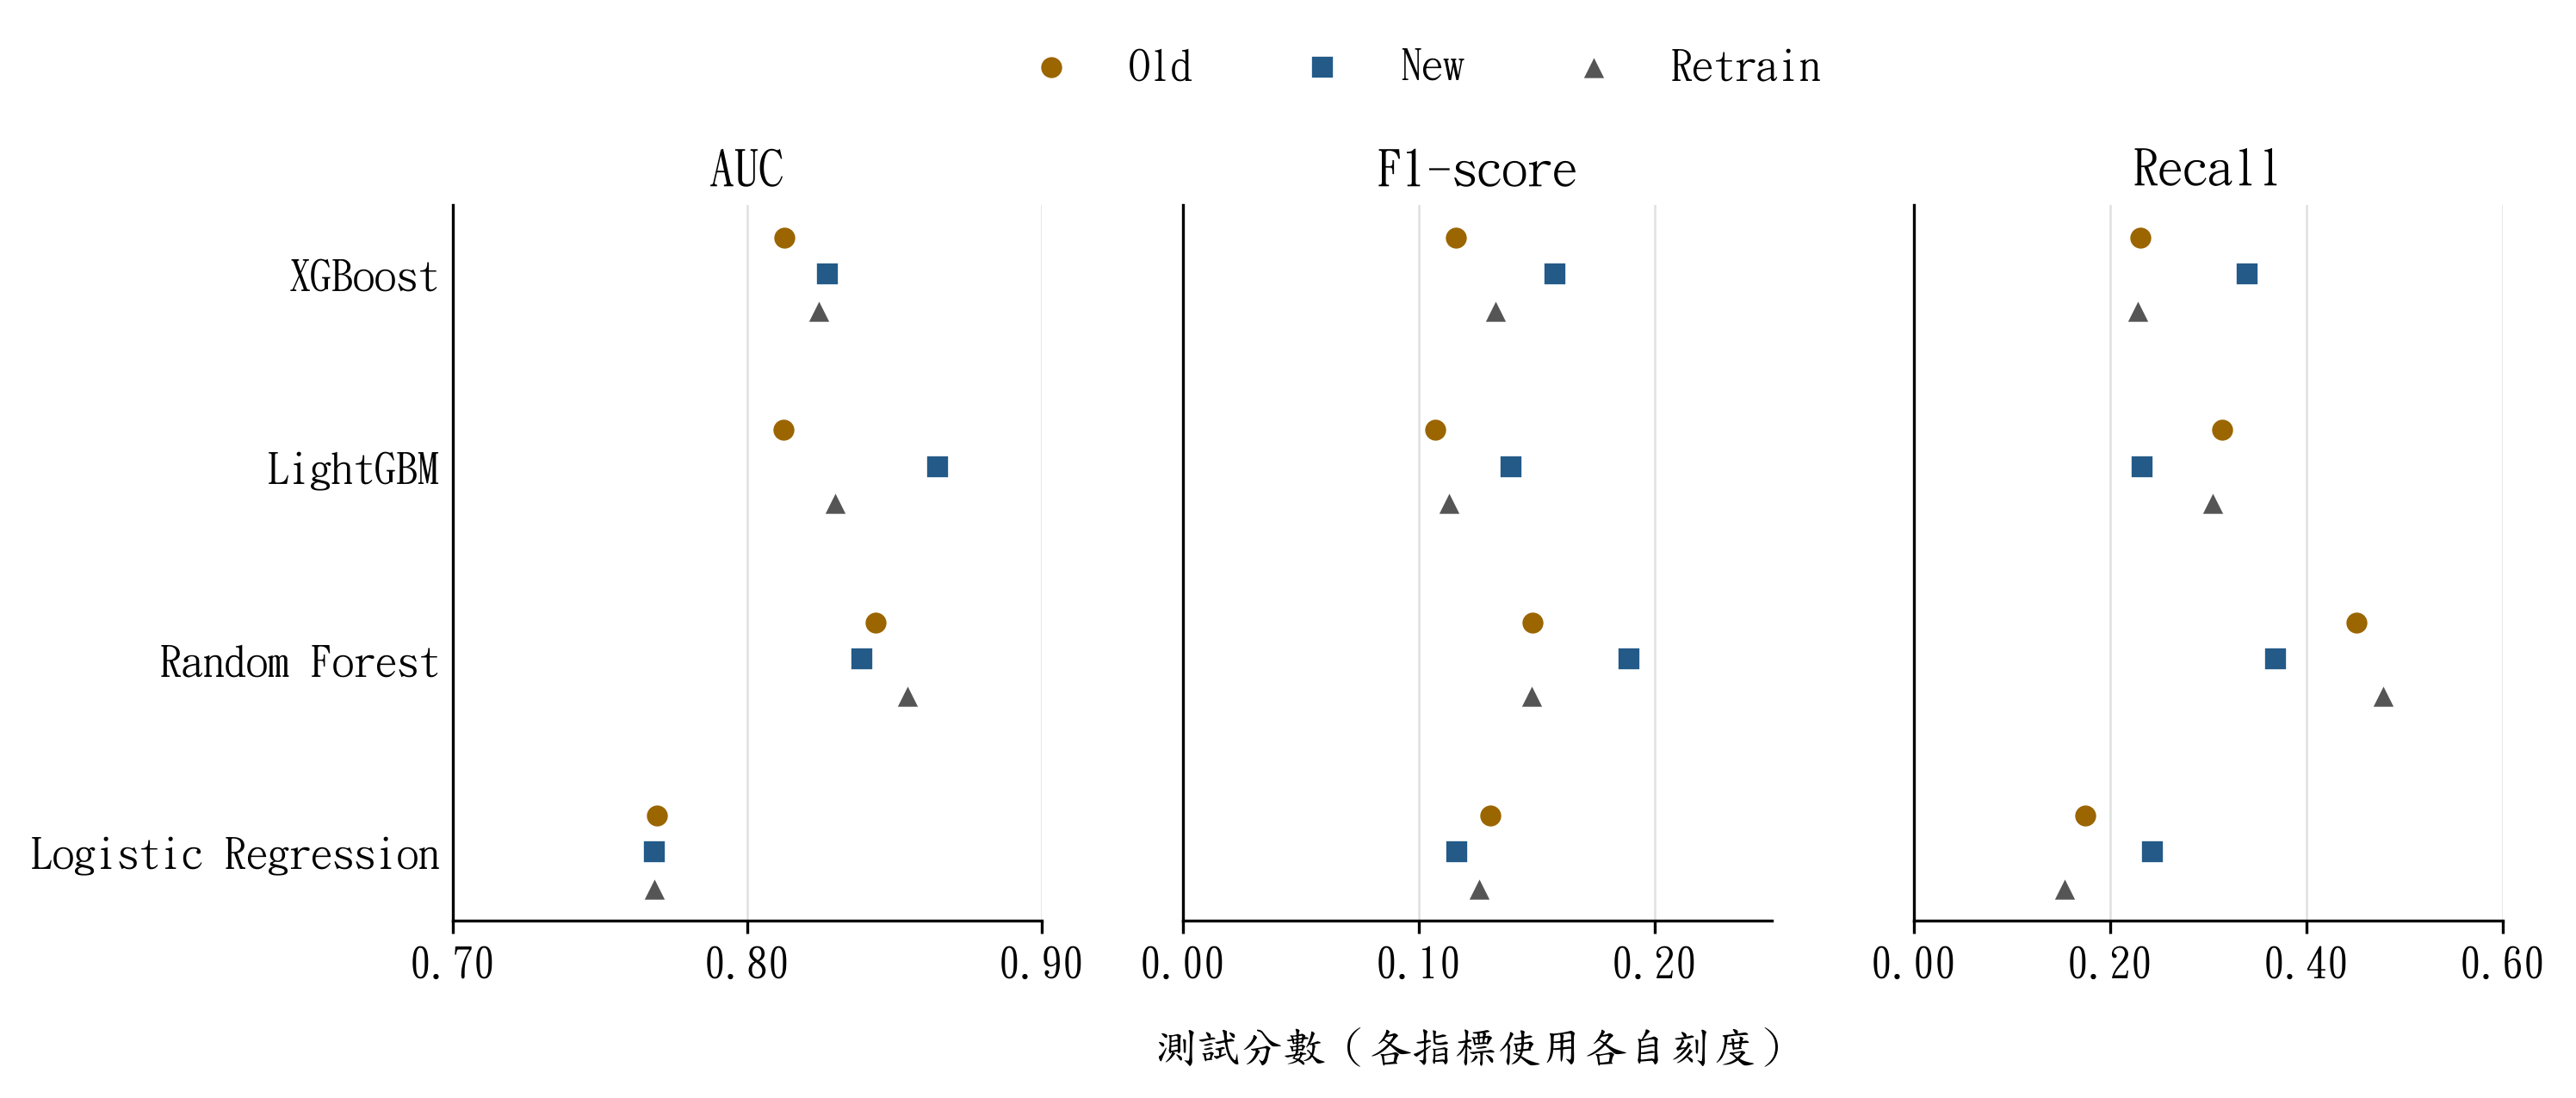
\includegraphics[width=\linewidth]{figures/event-baseline-strategies.png}
\caption{事件標籤下各分類器之訓練策略比較}\label{fig:results-baseline}
\par\smallskip{\footnotesize (資料來源：本研究依表~\ref{tab:results-baseline}之完整精度結果繪製)\par 各點為四種採樣與十個種子之平均。各指標刻度不同；點位不含信賴區間，分類器依固定順序排列。\par}
\end{figure}

近期資料的優勢並非在所有分類器都出現。XGBoost 與 LightGBM 的 New AUC 分別為 0.8272 與 0.8646，高於 Old 的 0.8125 與 0.8123；Random Forest 則以 Retrain 的 0.8543 最高，Old 的 0.8437 也高於 New 的 0.8389。Logistic Regression 三種策略的 AUC 都約為 0.769。F1-score 方面，XGBoost、LightGBM 與 Random Forest 都以 New 最高，Logistic Regression 則以 Old 最高。因此，資料期間的影響須與分類器一起判讀，不能概括為「近期資料一定較好」。

表~\ref{tab:results-classifier-validation} 只使用驗證資料，比較四種分類器在集成池六個位置上的表現。Random Forest 的驗證 AUC 為 0.8538，其次為 Logistic Regression 0.8330、XGBoost 0.8314 與 LightGBM 0.8260。Logistic Regression 的驗證排名較前，但 Test AUC 最低，可見只有 33 筆事件的驗證資料不足以穩定區分分類器。本研究不據此改換集成基底，也不宣稱 XGBoost 為最佳分類器。

\begingroup
\small\setstretch{1.12}\setlength{\tabcolsep}{3pt}
\setlength{\LTleft}{\fill}\setlength{\LTright}{\fill}
\Needspace{12\baselineskip}
\begin{longtable}{@{}>{\raggedright\arraybackslash}p{0.16\linewidth}>{\raggedright\arraybackslash}p{0.36\linewidth}>{\raggedright\arraybackslash}p{0.20\linewidth}>{\raggedright\arraybackslash}p{0.20\linewidth}@{}}
\caption{六個模型池位置之分類器驗證結果}\label{tab:results-classifier-validation}\\
\toprule
驗證排名 & 分類器 & 驗證 AUC & 驗證 PR-AUC \\
\midrule\endfirsthead
\multicolumn{4}{c}{表~\thetable（續）}\\
\toprule
驗證排名 & 分類器 & 驗證 AUC & 驗證 PR-AUC \\
\midrule\endhead
\midrule\multicolumn{4}{r}{續下頁}\\\endfoot
\bottomrule\endlastfoot
1 & Random Forest & 0.8538 & 0.0627 \\
2 & Logistic Regression & 0.8330 & 0.0677 \\
3 & XGBoost & 0.8314 & 0.0511 \\
4 & LightGBM & 0.8260 & 0.0451 \\
\end{longtable}
\noindent{\footnotesize (資料來源：本研究事件標籤 Baseline 實驗結果)\par 各值為 Old／New 與 Under、Over、Hybrid 共六個模型池位置、十個種子的 2014 年驗證平均，依驗證 AUC 排序；本表不使用 Test 分數。2014 年驗證資料只有 33 筆正類，排名差距須審慎解讀。}
\endgroup


\section{實驗一：Old／New 集成比較}\label{sec:results-experiment1}

\subsection{六個基礎模型與靜態成員數}

表~\ref{tab:results-pool-models} 為池內六個 XGBoost 模型的結果。三個 New 模型的 AUC 都約為 0.83；Old\_over 與 Old\_hybrid 只有 0.6844 與 0.6874，F1-score 也僅 0.0227 與 0.0260。Old\_under 的 AUC 為 0.7812，是三個 Old 模型中最高者。成員品質差異明顯，後續的集成結果應連同成員本身解讀。

\begingroup
\small\setstretch{1.12}\setlength{\tabcolsep}{3pt}
\setlength{\LTleft}{\fill}\setlength{\LTright}{\fill}
\Needspace{14\baselineskip}
\begin{longtable}{@{}>{\raggedright\arraybackslash}p{0.30\linewidth}>{\raggedright\arraybackslash}p{0.21\linewidth}>{\raggedright\arraybackslash}p{0.21\linewidth}>{\raggedright\arraybackslash}p{0.21\linewidth}@{}}
\caption{事件標籤下六個基礎模型之測試結果}\label{tab:results-pool-models}\\
\toprule
基礎模型 & AUC & F1-score & Recall \\
\midrule\endfirsthead
\multicolumn{4}{c}{表~\thetable（續）}\\
\toprule
基礎模型 & AUC & F1-score & Recall \\
\midrule\endhead
\midrule\multicolumn{4}{r}{續下頁}\\\endfoot
\bottomrule\endlastfoot
Old\_under & 0.7812 & 0.0948 & 0.3277 \\
Old\_over & 0.6844 & 0.0227 & 0.0202 \\
Old\_hybrid & 0.6874 & 0.0260 & 0.0244 \\
New\_under & 0.8311 & \textbf{0.2004} & \textbf{0.3950} \\
New\_over & 0.8285 & 0.1137 & 0.3580 \\
New\_hybrid & \textbf{0.8314} & 0.1279 & 0.2672 \\
\end{longtable}
\noindent{\footnotesize (資料來源：本研究事件標籤集成實驗結果)\par 完整 18 特徵、十個種子平均；under、over、hybrid 分別為 TomekLinks、ADASYN、SMOTEENN。粗體為六模型中該指標最高值，不表示差異達統計顯著；門檻由 Calibration 決定。}
\endgroup


\begingroup
\small\setstretch{1.12}\setlength{\tabcolsep}{3pt}
\setlength{\LTleft}{\fill}\setlength{\LTright}{\fill}
\Needspace{13\baselineskip}
\begin{longtable}{@{}>{\raggedright\arraybackslash}p{0.15\linewidth}>{\raggedright\arraybackslash}p{0.15\linewidth}>{\raggedright\arraybackslash}p{0.21\linewidth}>{\raggedright\arraybackslash}p{0.21\linewidth}>{\raggedright\arraybackslash}p{0.21\linewidth}@{}}
\caption{事件標籤下不同靜態成員數之候選平均結果}\label{tab:results-static-size}\\
\toprule
模型數 & 候選數 & AUC & F1-score & Recall \\
\midrule\endfirsthead
\multicolumn{5}{c}{表~\thetable（續）}\\
\toprule
模型數 & 候選數 & AUC & F1-score & Recall \\
\midrule\endhead
\midrule\multicolumn{5}{r}{續下頁}\\\endfoot
\bottomrule\endlastfoot
2 & 9 & 0.7846 & \textbf{0.1071} & 0.1898 \\
3 & 18 & 0.7850 & 0.0973 & \textbf{0.2265} \\
4 & 15 & 0.7859 & 0.0964 & 0.2222 \\
5 & 6 & 0.7866 & 0.1053 & 0.1763 \\
6 & 1 & \textbf{0.7881} & 0.1041 & 0.1941 \\
\end{longtable}
\noindent{\footnotesize (資料來源：本研究事件標籤集成實驗結果)\par 每個種子先平均同一成員數全部候選的 Test 分數，再取十個種子平均。粗體僅供比較，不依此選成員數，也不表示顯著差異。}
\endgroup


表~\ref{tab:results-static-size} 依成員數平均 49 個混合候選。兩模型到六模型候選的平均 AUC 介於 0.7846 與 0.7881，差距很小；這些平均涵蓋不同組合，不能解釋為只改變成員數的效果。V-static 仍由 Calibration AP 選擇，不依本表決定成員數。

\subsection{集成方法比較}

表~\ref{tab:results-ensemble} 與圖~\ref{fig:results-ensemble} 比較八種集成方法。Old3 與 New3 各整合同一期間的三個模型，Equal6 平均全部六模型，V-static 依各種子的 Calibration AP 從 49 個混合子集選定成員；四種動態方法使用相同模型池與 DSEL。

\begingroup
\small\setstretch{1.12}\setlength{\tabcolsep}{3pt}
\setlength{\LTleft}{\fill}\setlength{\LTright}{\fill}
\Needspace{24\baselineskip}
\begin{longtable}{@{}>{\raggedright\arraybackslash}p{0.16\linewidth}>{\raggedright\arraybackslash}p{0.18\linewidth}>{\raggedright\arraybackslash}p{0.18\linewidth}>{\raggedright\arraybackslash}p{0.18\linewidth}>{\raggedright\arraybackslash}p{0.18\linewidth}@{}}
\caption{事件標籤下未進行 FS 之集成方法結果}\label{tab:results-ensemble}\\
\toprule
方法 & AUC & PR-AUC & F1-score & Recall \\
\midrule\endfirsthead
\multicolumn{5}{c}{表~\thetable（續）}\\
\toprule
方法 & AUC & PR-AUC & F1-score & Recall \\
\midrule\endhead
\midrule\multicolumn{5}{r}{續下頁}\\\endfoot
\bottomrule\endlastfoot
Old3 & \shortstack[l]{0.7198\\{\scriptsize(\(\pm\)0.0062)}} & \shortstack[l]{0.0245\\{\scriptsize(\(\pm\)0.0009)}} & \shortstack[l]{0.0199\\{\scriptsize(\(\pm\)0.0146)}} & \shortstack[l]{0.0168\\{\scriptsize(\(\pm\)0.0137)}} \\
New3 & \shortstack[l]{\textbf{0.8601}\\{\scriptsize(\(\pm\)0.0043)}} & \shortstack[l]{0.0905\\{\scriptsize(\(\pm\)0.0055)}} & \shortstack[l]{0.1289\\{\scriptsize(\(\pm\)0.0142)}} & \shortstack[l]{0.4319\\{\scriptsize(\(\pm\)0.0605)}} \\
Equal6 & \shortstack[l]{0.7881\\{\scriptsize(\(\pm\)0.0037)}} & \shortstack[l]{0.0533\\{\scriptsize(\(\pm\)0.0027)}} & \shortstack[l]{0.1041\\{\scriptsize(\(\pm\)0.0073)}} & \shortstack[l]{0.1941\\{\scriptsize(\(\pm\)0.0535)}} \\
V-static & \shortstack[l]{0.8472\\{\scriptsize(\(\pm\)0.0000)}} & \shortstack[l]{\textbf{0.1252}\\{\scriptsize(\(\pm\)0.0000)}} & \shortstack[l]{\textbf{0.1795}\\{\scriptsize(\(\pm\)0.0000)}} & \shortstack[l]{0.2353\\{\scriptsize(\(\pm\)0.0000)}} \\
DCS-OLA & \shortstack[l]{0.7450\\{\scriptsize(\(\pm\)0.0079)}} & \shortstack[l]{0.0288\\{\scriptsize(\(\pm\)0.0025)}} & \shortstack[l]{0.0411\\{\scriptsize(\(\pm\)0.0167)}} & \shortstack[l]{0.3857\\{\scriptsize(\(\pm\)0.2526)}} \\
DCS-LCA & \shortstack[l]{0.7450\\{\scriptsize(\(\pm\)0.0082)}} & \shortstack[l]{0.0298\\{\scriptsize(\(\pm\)0.0032)}} & \shortstack[l]{0.0404\\{\scriptsize(\(\pm\)0.0185)}} & \shortstack[l]{0.3849\\{\scriptsize(\(\pm\)0.2540)}} \\
KNORA-E & \shortstack[l]{0.7859\\{\scriptsize(\(\pm\)0.0052)}} & \shortstack[l]{0.0581\\{\scriptsize(\(\pm\)0.0049)}} & \shortstack[l]{0.1017\\{\scriptsize(\(\pm\)0.0297)}} & \shortstack[l]{0.2739\\{\scriptsize(\(\pm\)0.2164)}} \\
KNORA-U & \shortstack[l]{0.7771\\{\scriptsize(\(\pm\)0.0045)}} & \shortstack[l]{0.0513\\{\scriptsize(\(\pm\)0.0039)}} & \shortstack[l]{0.0686\\{\scriptsize(\(\pm\)0.0268)}} & \shortstack[l]{\textbf{0.4824}\\{\scriptsize(\(\pm\)0.2116)}} \\
\end{longtable}
\noindent{\footnotesize (資料來源：本研究事件標籤集成實驗結果)\par 各格上列為十個種子之合併四年 Test 平均，下列為種子標準差；Test 共 12,282 筆紀錄、119 筆事件。粗體為八種方法中該指標最高值，不表示差異達統計顯著。}
\endgroup


\begin{figure}[htbp]
\centering
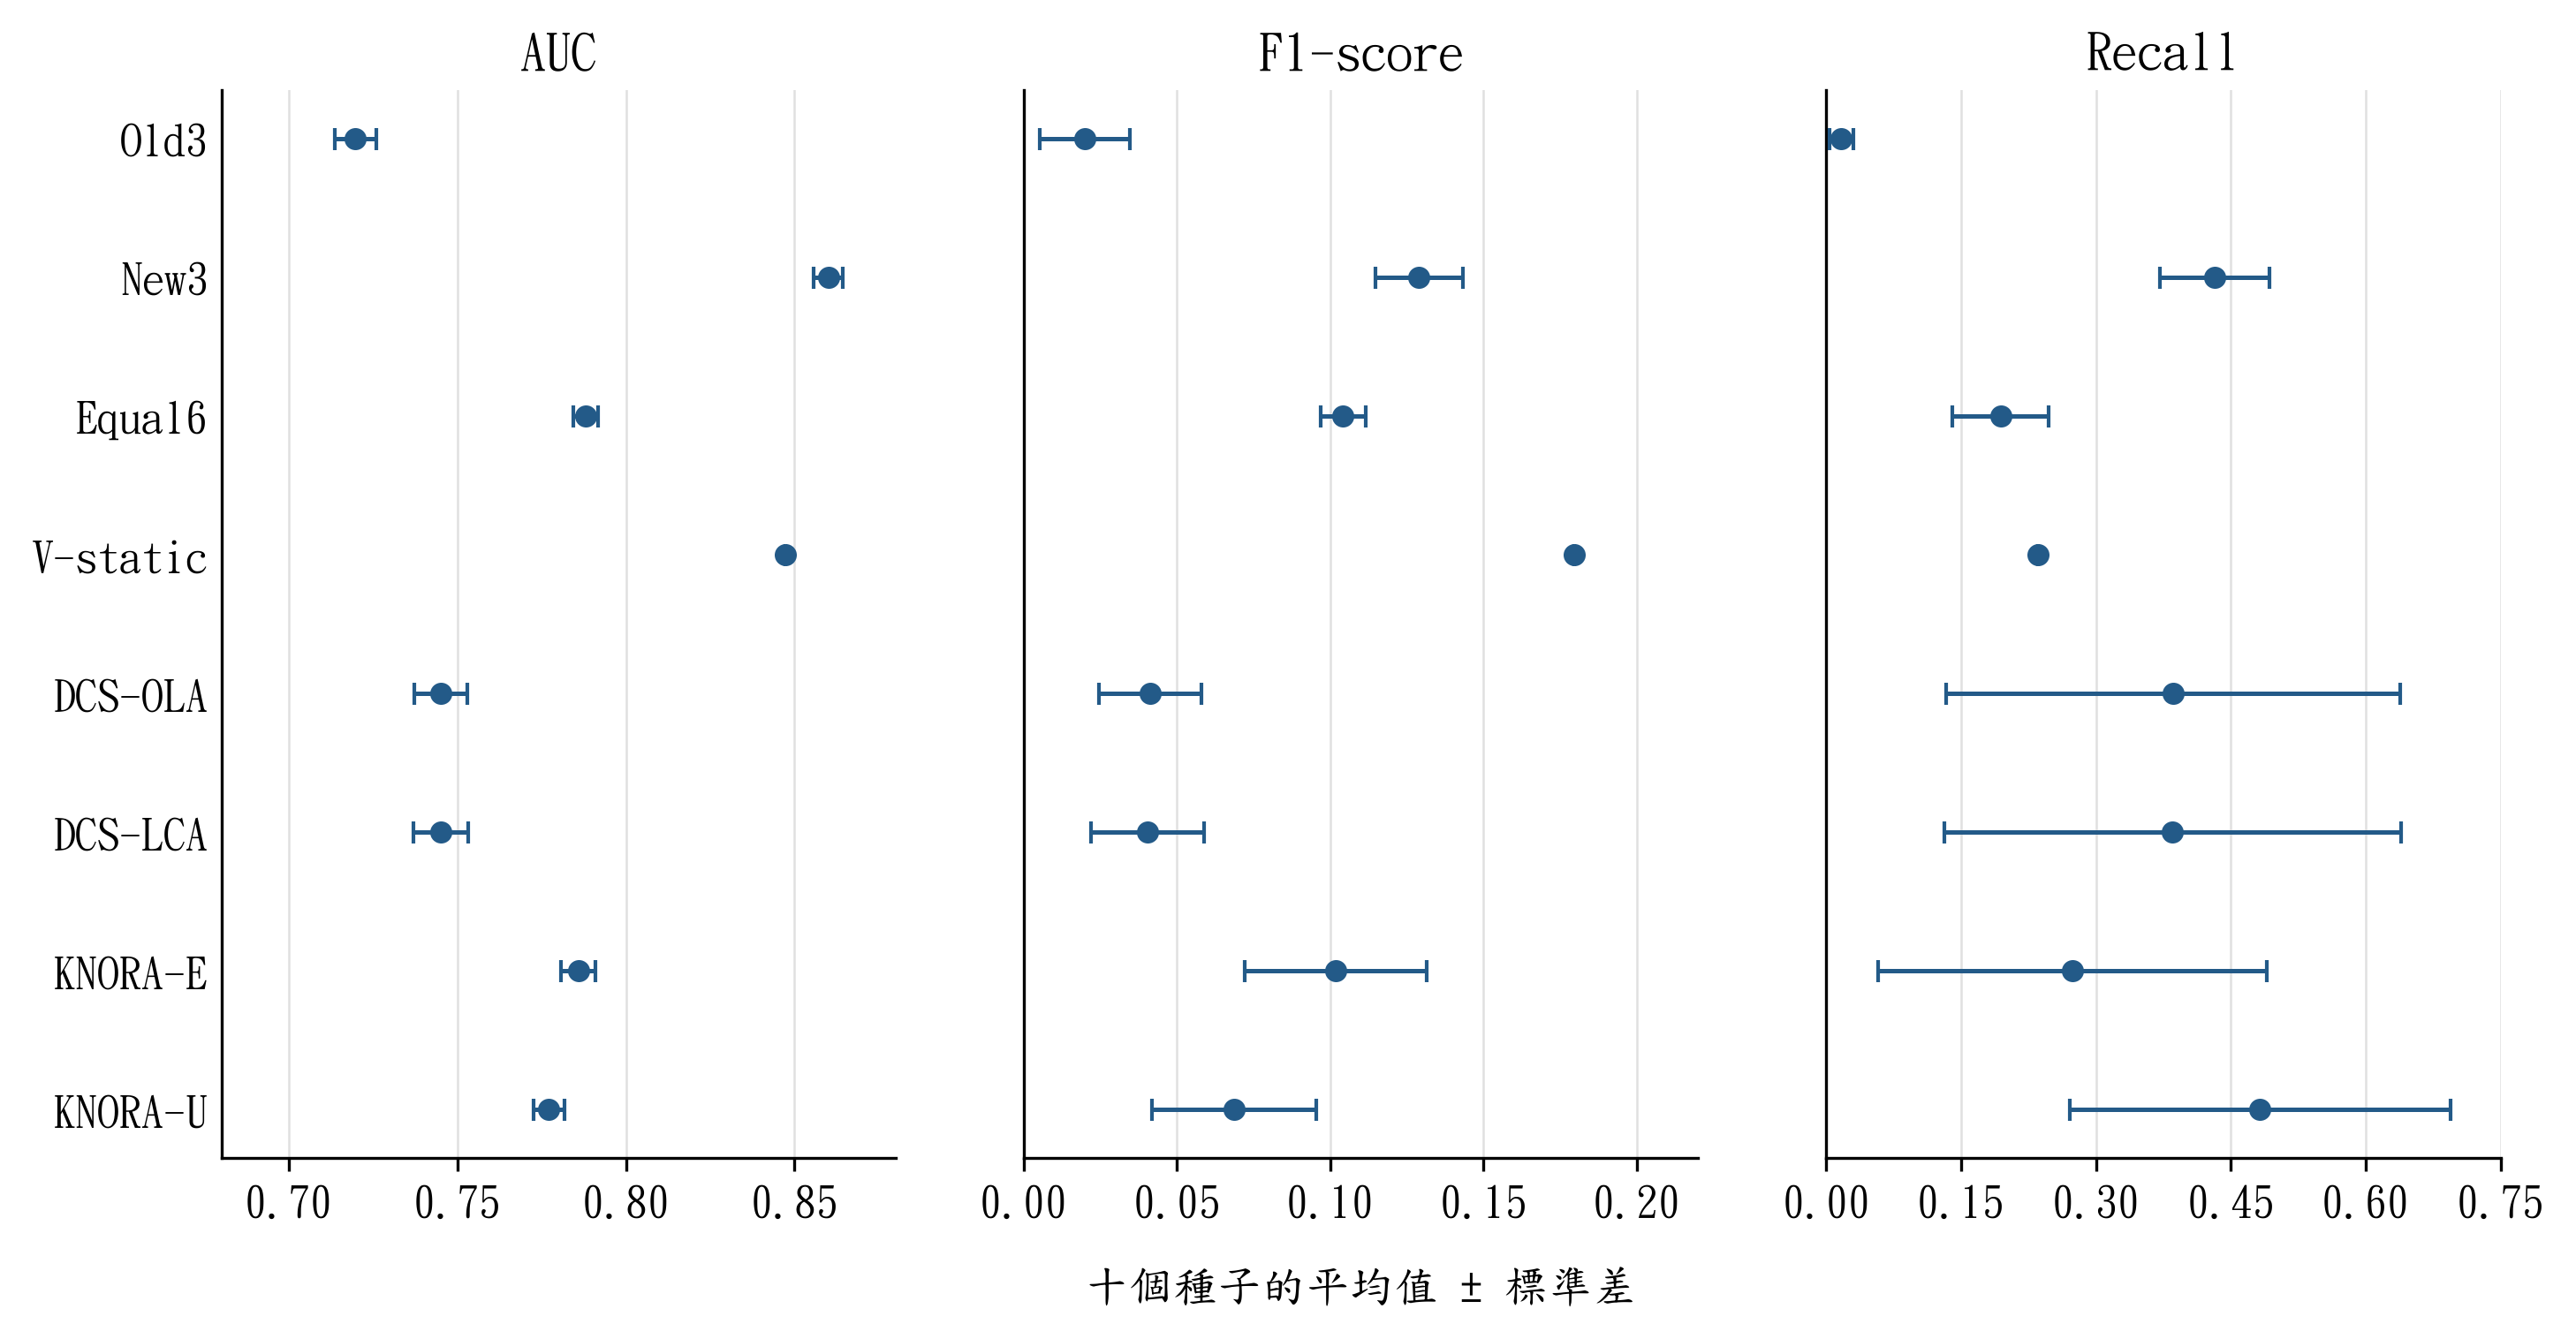
\includegraphics[width=\linewidth]{figures/event-ensemble-comparison.png}
\caption{事件標籤下未進行 FS 之集成方法比較}\label{fig:results-ensemble}
\par\smallskip{\footnotesize (資料來源：本研究事件標籤集成實驗結果)\par 點為合併四年測試指標的十種子平均，線段為種子標準差，並非公司重抽樣的信賴區間。各指標刻度不同，方法順序不依測試分數排列。\par}
\end{figure}

New3 的平均 AUC 最高，為 0.8601；V-static 為 0.8472，但 PR-AUC 與 F1-score 最高，分別為 0.1252 與 0.1795。十個種子的 V-static 都選中 Old\_under 與 New\_under 兩個模型，等於只保留各期間表現最好的一個成員。相對地，Equal6 的 AUC 為 0.7881，低於 New3，顯示把兩個較弱的 Old 模型一起等權平均，會拉低整體排序能力。Old3 的 F1-score 與 Recall 僅 0.0199 與 0.0168，幾乎無法辨識事件。

動態方法沒有超過 New3 或 V-static。DCS-OLA 與 DCS-LCA 的 AUC 都是 0.7450；KNORA-E 為 0.7859，與 Equal6 相近。KNORA-U 與兩種 DCS 的平均 Recall 雖高於 0.38，但種子標準差超過 0.21，F1-score 也偏低，代表判為事件的紀錄中誤報很多，且結果隨種子變動大。

綜合而言，在固定的六模型池中，「選擇哪些成員」比「是否整合全部成員」更影響結果：只用近期模型的 New3 與只選兩個成員的 V-static 表現較佳，全部等權平均與動態選擇則未帶來改善。這些差異尚未經事件標籤的配對檢定，屬描述性觀察。

\subsection{與 Baseline 的公平比較}

集成池的六個 XGBoost 使用預設參數，即 Baseline 搜尋中的候選 0；Baseline 則從 24 組候選中選參。表~\ref{tab:results-tuning-gap} 以相同資料列、標籤、擬合期間與採樣對照兩者。

\begingroup
\small\setstretch{1.12}\setlength{\tabcolsep}{3pt}
\setlength{\LTleft}{\fill}\setlength{\LTright}{\fill}
\Needspace{20\baselineskip}
\begin{longtable}{@{}>{\raggedright\arraybackslash}p{0.20\linewidth}>{\raggedright\arraybackslash}p{0.26\linewidth}>{\raggedright\arraybackslash}p{0.16\linewidth}>{\raggedright\arraybackslash}p{0.16\linewidth}>{\raggedright\arraybackslash}p{0.16\linewidth}@{}}
\caption{集成池預設 XGBoost 與 Baseline 調參 XGBoost 之對照}\label{tab:results-tuning-gap}\\
\toprule
模型池位置 & XGBoost 參數 & AUC & F1-score & Recall \\
\midrule\endfirsthead
\multicolumn{5}{c}{表~\thetable（續）}\\
\toprule
模型池位置 & XGBoost 參數 & AUC & F1-score & Recall \\
\midrule\endhead
\midrule\multicolumn{5}{r}{續下頁}\\\endfoot
\bottomrule\endlastfoot
Old\_under & 預設（集成池） & 0.7812 & 0.0948 & 0.3277 \\
 & 調參（候選 5） & 0.8710 & 0.1590 & 0.2748 \\
Old\_over & 預設（集成池） & 0.6844 & 0.0227 & 0.0202 \\
 & 調參（候選 4） & 0.7532 & 0.0755 & 0.1630 \\
Old\_hybrid & 預設（集成池） & 0.6874 & 0.0260 & 0.0244 \\
 & 調參（候選 4） & 0.7544 & 0.0746 & 0.1731 \\
New\_under & 預設（集成池） & 0.8311 & 0.2004 & 0.3950 \\
 & 調參（候選 20） & 0.7965 & 0.1595 & 0.3109 \\
New\_over & 預設（集成池） & 0.8285 & 0.1137 & 0.3580 \\
 & 調參（候選 13） & 0.8577 & 0.1463 & 0.3689 \\
New\_hybrid & 預設（集成池） & 0.8314 & 0.1279 & 0.2672 \\
 & 調參（候選 13） & 0.8577 & 0.1598 & 0.3496 \\
\end{longtable}
\noindent{\footnotesize (資料來源：本研究事件標籤集成與 Baseline 實驗結果)\par 兩者使用相同資料列、標籤、擬合期間與採樣；預設列的門檻由 Calibration（2014 年半數）決定，調參列的參數與門檻由完整 2014 年驗證資料決定。各值為十個種子的合併四年 Test 平均，僅供說明參數條件的差異。}
\endgroup


調參在五個位置提高 AUC，例如 Old\_under 由 0.7812 提高到 0.8710，Old\_hybrid 由 0.6874 提高到 0.7544；New\_under 則由 0.8311 降為 0.7965，表示依 33 筆事件選出的參數未必在 Test 較好。調參後的單一模型也與集成相當，例如 LightGBM New 的平均 AUC 為 0.8646，Random Forest Retrain 為 0.8543，均不低於 V-static 的 0.8472。

因此，Baseline 與集成之間的分數差同時包含參數、驗證資料（完整 2014 年或其中一半）與分類器的差異，不能全部歸因於集成本身。本研究可以比較的是同一模型池內的整合方式；集成能否優於調參後的單一分類器，需要以調參後的成員重建模型池才能回答。

\subsection{不同測試年度的表現}

\begingroup
\small\setstretch{1.12}\setlength{\tabcolsep}{3pt}
\setlength{\LTleft}{\fill}\setlength{\LTright}{\fill}
\begin{longtable}{@{}>{\raggedright\arraybackslash}p{0.28\linewidth}>{\raggedright\arraybackslash}p{0.12\linewidth}>{\raggedright\arraybackslash}p{0.18\linewidth}>{\raggedright\arraybackslash}p{0.18\linewidth}>{\raggedright\arraybackslash}p{0.18\linewidth}@{}}
\caption{事件標籤下固定年份集成之逐年測試結果}\label{tab:results-ensemble-yearly}\\
\toprule
方法 & 年度 & AUC & F1-score & Recall \\
\midrule\endfirsthead
\multicolumn{5}{c}{表~\thetable（續）}\\
\toprule
方法 & 年度 & AUC & F1-score & Recall \\
\midrule\endhead
\midrule\multicolumn{5}{r}{續下頁}\\\endfoot
\bottomrule\endlastfoot
\multirow[t]{4}{=}{Old3} & 2015 & 0.6958 & 0.0292 & 0.0242 \\*
 & 2016 & 0.6817 & 0.0080 & 0.0069 \\*
 & 2017 & 0.7861 & 0.0000 & 0.0000 \\*
 & 2018 & 0.7345 & 0.0381 & 0.0278 \\
\addlinespace[4pt]
\multirow[t]{4}{=}{New3} & 2015 & \textbf{0.8721} & 0.1423 & 0.4818 \\*
 & 2016 & \textbf{0.8479} & 0.1328 & \textbf{0.4517} \\*
 & 2017 & 0.8792 & 0.0963 & 0.4238 \\*
 & 2018 & 0.8465 & 0.1412 & 0.3750 \\
\addlinespace[4pt]
\multirow[t]{4}{=}{Equal6} & 2015 & 0.7696 & \textbf{0.1575} & 0.2909 \\*
 & 2016 & 0.7450 & 0.0858 & 0.1793 \\*
 & 2017 & 0.8464 & 0.0513 & 0.1286 \\*
 & 2018 & 0.8072 & 0.1061 & 0.1556 \\
\addlinespace[4pt]
\multirow[t]{4}{=}{V-static} & 2015 & 0.8291 & 0.1463 & 0.1818 \\*
 & 2016 & 0.8117 & \textbf{0.1772} & 0.2414 \\*
 & 2017 & \textbf{0.8917} & \textbf{0.2388} & 0.3810 \\*
 & 2018 & \textbf{0.8651} & \textbf{0.1667} & 0.1944 \\
\addlinespace[4pt]
\multirow[t]{4}{=}{DCS-OLA} & 2015 & 0.6833 & 0.0355 & 0.3182 \\*
 & 2016 & 0.7069 & 0.0418 & 0.3759 \\*
 & 2017 & 0.8184 & 0.0361 & 0.4810 \\*
 & 2018 & 0.7897 & 0.0529 & 0.4000 \\
\addlinespace[4pt]
\multirow[t]{4}{=}{DCS-LCA} & 2015 & 0.6817 & 0.0311 & 0.3152 \\*
 & 2016 & 0.7074 & 0.0426 & 0.3759 \\*
 & 2017 & 0.8192 & 0.0365 & 0.4810 \\*
 & 2018 & 0.7902 & 0.0532 & 0.4000 \\
\addlinespace[4pt]
\multirow[t]{4}{=}{KNORA-E} & 2015 & 0.7709 & 0.1574 & 0.3455 \\*
 & 2016 & 0.7454 & 0.0891 & 0.2483 \\*
 & 2017 & 0.8416 & 0.0480 & 0.2429 \\*
 & 2018 & 0.7996 & 0.0996 & 0.2472 \\
\addlinespace[4pt]
\multirow[t]{4}{=}{KNORA-U} & 2015 & 0.7612 & 0.0870 & \textbf{0.5121} \\*
 & 2016 & 0.7351 & 0.0628 & 0.4483 \\*
 & 2017 & 0.8164 & 0.0452 & \textbf{0.5000} \\*
 & 2018 & 0.8038 & 0.0748 & \textbf{0.4722} \\
\end{longtable}
\noindent{\footnotesize (資料來源：本研究事件標籤集成實驗結果)\par 各值為十個種子的年度指標平均；粗體表示同一年度八種方法中該指標最高值。2015--2018 年事件數依序為 33、29、21、36；各年沿用 Calibration 固定的門檻。}
\endgroup


表~\ref{tab:results-ensemble-yearly} 分開列出四個測試年度。New3 在 2015 與 2016 年的 AUC 最高，V-static 則在 2017 與 2018 年最高，分別為 0.8917 與 0.8651。各年只有 21 至 36 筆事件，年度間的排名變動可能受少數樣本影響；本表不把四年當成四次獨立實驗，也不據此推論特定景氣因素。

\section{實驗二：FS 集成比較}\label{sec:results-experiment2}

八種 FS 條件分別與相同種子、測試樣本及集成方法的 no-FS 結果配對。50\% 與 80\% 分別保留 9 與 14 個特徵，精簡率為 50.00\% 與 22.22\%；各條件都重新訓練模型，並依相同 Calibration 規則決定成員與門檻。表~\ref{tab:results-fs-auc}、表~\ref{tab:results-fs-f1} 與表~\ref{tab:results-fs-recall} 列出完整結果。

\begingroup
\small\setstretch{1.12}\setlength{\tabcolsep}{3pt}
\setlength{\LTleft}{\fill}\setlength{\LTright}{\fill}
\Needspace{26\baselineskip}
\begin{longtable}{@{}>{\raggedright\arraybackslash}p{0.16\linewidth}>{\raggedright\arraybackslash}p{0.123\linewidth}>{\raggedright\arraybackslash}p{0.123\linewidth}>{\raggedright\arraybackslash}p{0.123\linewidth}>{\raggedright\arraybackslash}p{0.123\linewidth}>{\raggedright\arraybackslash}p{0.123\linewidth}>{\raggedright\arraybackslash}p{0.123\linewidth}@{}}
\caption{事件標籤下實驗二各特徵條件之 AUC}\label{tab:results-fs-auc}\\
\toprule
FS & Equal6 & V-static & OLA & LCA & KNORA-E & KNORA-U \\
\midrule\endfirsthead
\multicolumn{7}{c}{表~\thetable（續）}\\
\toprule
FS & Equal6 & V-static & OLA & LCA & KNORA-E & KNORA-U \\
\midrule\endhead
\midrule\multicolumn{7}{r}{續下頁}\\\endfoot
\bottomrule\endlastfoot
no-FS（18） & \shortstack[l]{0.7881\\{\scriptsize(\(\pm\)0.0037)}} & \shortstack[l]{0.8472\\{\scriptsize(\(\pm\)0.0000)}} & \shortstack[l]{\textbf{0.7450}\\{\scriptsize(\(\pm\)0.0079)}} & \shortstack[l]{\textbf{0.7450}\\{\scriptsize(\(\pm\)0.0082)}} & \shortstack[l]{0.7859\\{\scriptsize(\(\pm\)0.0052)}} & \shortstack[l]{0.7771\\{\scriptsize(\(\pm\)0.0045)}} \\
MI 50\% & \shortstack[l]{0.7827\\{\scriptsize(\(\pm\)0.0075)}} & \shortstack[l]{0.8440\\{\scriptsize(\(\pm\)0.0311)}} & \shortstack[l]{0.7180\\{\scriptsize(\(\pm\)0.0161)}} & \shortstack[l]{0.7148\\{\scriptsize(\(\pm\)0.0133)}} & \shortstack[l]{0.7674\\{\scriptsize(\(\pm\)0.0071)}} & \shortstack[l]{0.7622\\{\scriptsize(\(\pm\)0.0068)}} \\
MI 80\% & \shortstack[l]{0.7902\\{\scriptsize(\(\pm\)0.0043)}} & \shortstack[l]{0.8573\\{\scriptsize(\(\pm\)0.0036)}} & \shortstack[l]{0.7329\\{\scriptsize(\(\pm\)0.0122)}} & \shortstack[l]{0.7329\\{\scriptsize(\(\pm\)0.0119)}} & \shortstack[l]{0.7795\\{\scriptsize(\(\pm\)0.0065)}} & \shortstack[l]{0.7776\\{\scriptsize(\(\pm\)0.0068)}} \\
CART 50\% & \shortstack[l]{0.7748\\{\scriptsize(\(\pm\)0.0045)}} & \shortstack[l]{0.8523\\{\scriptsize(\(\pm\)0.0000)}} & \shortstack[l]{0.7139\\{\scriptsize(\(\pm\)0.0076)}} & \shortstack[l]{0.7143\\{\scriptsize(\(\pm\)0.0078)}} & \shortstack[l]{0.7559\\{\scriptsize(\(\pm\)0.0073)}} & \shortstack[l]{0.7603\\{\scriptsize(\(\pm\)0.0066)}} \\
CART 80\% & \shortstack[l]{0.7736\\{\scriptsize(\(\pm\)0.0049)}} & \shortstack[l]{0.8492\\{\scriptsize(\(\pm\)0.0023)}} & \shortstack[l]{0.7368\\{\scriptsize(\(\pm\)0.0084)}} & \shortstack[l]{0.7373\\{\scriptsize(\(\pm\)0.0082)}} & \shortstack[l]{0.7673\\{\scriptsize(\(\pm\)0.0052)}} & \shortstack[l]{0.7640\\{\scriptsize(\(\pm\)0.0072)}} \\
SHAP 50\% & \shortstack[l]{0.7565\\{\scriptsize(\(\pm\)0.0059)}} & \shortstack[l]{0.7885\\{\scriptsize(\(\pm\)0.0498)}} & \shortstack[l]{0.6995\\{\scriptsize(\(\pm\)0.0083)}} & \shortstack[l]{0.6980\\{\scriptsize(\(\pm\)0.0082)}} & \shortstack[l]{0.7520\\{\scriptsize(\(\pm\)0.0040)}} & \shortstack[l]{0.7496\\{\scriptsize(\(\pm\)0.0076)}} \\
SHAP 80\% & \shortstack[l]{\textbf{0.7906}\\{\scriptsize(\(\pm\)0.0065)}} & \shortstack[l]{0.8512\\{\scriptsize(\(\pm\)0.0000)}} & \shortstack[l]{0.7396\\{\scriptsize(\(\pm\)0.0092)}} & \shortstack[l]{0.7390\\{\scriptsize(\(\pm\)0.0088)}} & \shortstack[l]{\textbf{0.7920}\\{\scriptsize(\(\pm\)0.0073)}} & \shortstack[l]{\textbf{0.7878}\\{\scriptsize(\(\pm\)0.0072)}} \\
RFE 50\% & \shortstack[l]{0.7759\\{\scriptsize(\(\pm\)0.0045)}} & \shortstack[l]{0.8523\\{\scriptsize(\(\pm\)0.0000)}} & \shortstack[l]{0.7159\\{\scriptsize(\(\pm\)0.0096)}} & \shortstack[l]{0.7161\\{\scriptsize(\(\pm\)0.0093)}} & \shortstack[l]{0.7583\\{\scriptsize(\(\pm\)0.0066)}} & \shortstack[l]{0.7633\\{\scriptsize(\(\pm\)0.0063)}} \\
RFE 80\% & \shortstack[l]{0.7844\\{\scriptsize(\(\pm\)0.0049)}} & \shortstack[l]{\textbf{0.8579}\\{\scriptsize(\(\pm\)0.0000)}} & \shortstack[l]{0.7339\\{\scriptsize(\(\pm\)0.0069)}} & \shortstack[l]{0.7310\\{\scriptsize(\(\pm\)0.0075)}} & \shortstack[l]{0.7741\\{\scriptsize(\(\pm\)0.0036)}} & \shortstack[l]{0.7702\\{\scriptsize(\(\pm\)0.0057)}} \\
\end{longtable}
\noindent{\footnotesize (資料來源：本研究事件標籤 FS 集成實驗結果)\par 各格上列為十個種子的合併四年 Test 平均，下列為種子標準差。粗體表示同一方法（同一欄）九種特徵條件中最高的平均分數，不代表已選定最佳設定或差異達統計顯著。50\%、80\% 分別保留 9、14 個特徵；V-static 依各條件的 Calibration 重新選成員。}
\endgroup

\begingroup
\small\setstretch{1.12}\setlength{\tabcolsep}{3pt}
\setlength{\LTleft}{\fill}\setlength{\LTright}{\fill}
\Needspace{26\baselineskip}
\begin{longtable}{@{}>{\raggedright\arraybackslash}p{0.16\linewidth}>{\raggedright\arraybackslash}p{0.123\linewidth}>{\raggedright\arraybackslash}p{0.123\linewidth}>{\raggedright\arraybackslash}p{0.123\linewidth}>{\raggedright\arraybackslash}p{0.123\linewidth}>{\raggedright\arraybackslash}p{0.123\linewidth}>{\raggedright\arraybackslash}p{0.123\linewidth}@{}}
\caption{事件標籤下實驗二各特徵條件之 F1-score}\label{tab:results-fs-f1}\\
\toprule
FS & Equal6 & V-static & OLA & LCA & KNORA-E & KNORA-U \\
\midrule\endfirsthead
\multicolumn{7}{c}{表~\thetable（續）}\\
\toprule
FS & Equal6 & V-static & OLA & LCA & KNORA-E & KNORA-U \\
\midrule\endhead
\midrule\multicolumn{7}{r}{續下頁}\\\endfoot
\bottomrule\endlastfoot
no-FS（18） & \shortstack[l]{0.1041\\{\scriptsize(\(\pm\)0.0073)}} & \shortstack[l]{\textbf{0.1795}\\{\scriptsize(\(\pm\)0.0000)}} & \shortstack[l]{0.0411\\{\scriptsize(\(\pm\)0.0167)}} & \shortstack[l]{0.0404\\{\scriptsize(\(\pm\)0.0185)}} & \shortstack[l]{0.1017\\{\scriptsize(\(\pm\)0.0297)}} & \shortstack[l]{0.0686\\{\scriptsize(\(\pm\)0.0268)}} \\
MI 50\% & \shortstack[l]{0.0886\\{\scriptsize(\(\pm\)0.0200)}} & \shortstack[l]{0.1421\\{\scriptsize(\(\pm\)0.0384)}} & \shortstack[l]{0.0478\\{\scriptsize(\(\pm\)0.0081)}} & \shortstack[l]{0.0448\\{\scriptsize(\(\pm\)0.0095)}} & \shortstack[l]{0.0934\\{\scriptsize(\(\pm\)0.0260)}} & \shortstack[l]{0.0736\\{\scriptsize(\(\pm\)0.0270)}} \\
MI 80\% & \shortstack[l]{0.1028\\{\scriptsize(\(\pm\)0.0228)}} & \shortstack[l]{0.1715\\{\scriptsize(\(\pm\)0.0410)}} & \shortstack[l]{0.0502\\{\scriptsize(\(\pm\)0.0204)}} & \shortstack[l]{0.0504\\{\scriptsize(\(\pm\)0.0211)}} & \shortstack[l]{0.1035\\{\scriptsize(\(\pm\)0.0290)}} & \shortstack[l]{0.0728\\{\scriptsize(\(\pm\)0.0302)}} \\
CART 50\% & \shortstack[l]{0.0867\\{\scriptsize(\(\pm\)0.0127)}} & \shortstack[l]{0.1444\\{\scriptsize(\(\pm\)0.0000)}} & \shortstack[l]{0.0341\\{\scriptsize(\(\pm\)0.0212)}} & \shortstack[l]{0.0356\\{\scriptsize(\(\pm\)0.0204)}} & \shortstack[l]{0.0972\\{\scriptsize(\(\pm\)0.0220)}} & \shortstack[l]{0.0819\\{\scriptsize(\(\pm\)0.0169)}} \\
CART 80\% & \shortstack[l]{0.0976\\{\scriptsize(\(\pm\)0.0158)}} & \shortstack[l]{0.1736\\{\scriptsize(\(\pm\)0.0077)}} & \shortstack[l]{\textbf{0.0676}\\{\scriptsize(\(\pm\)0.0119)}} & \shortstack[l]{\textbf{0.0664}\\{\scriptsize(\(\pm\)0.0114)}} & \shortstack[l]{\textbf{0.1112}\\{\scriptsize(\(\pm\)0.0244)}} & \shortstack[l]{\textbf{0.0955}\\{\scriptsize(\(\pm\)0.0311)}} \\
SHAP 50\% & \shortstack[l]{\textbf{0.1325}\\{\scriptsize(\(\pm\)0.0237)}} & \shortstack[l]{0.1396\\{\scriptsize(\(\pm\)0.0268)}} & \shortstack[l]{0.0441\\{\scriptsize(\(\pm\)0.0182)}} & \shortstack[l]{0.0367\\{\scriptsize(\(\pm\)0.0144)}} & \shortstack[l]{0.0743\\{\scriptsize(\(\pm\)0.0269)}} & \shortstack[l]{0.0938\\{\scriptsize(\(\pm\)0.0269)}} \\
SHAP 80\% & \shortstack[l]{0.0755\\{\scriptsize(\(\pm\)0.0395)}} & \shortstack[l]{0.1566\\{\scriptsize(\(\pm\)0.0000)}} & \shortstack[l]{0.0515\\{\scriptsize(\(\pm\)0.0084)}} & \shortstack[l]{0.0500\\{\scriptsize(\(\pm\)0.0061)}} & \shortstack[l]{0.0910\\{\scriptsize(\(\pm\)0.0434)}} & \shortstack[l]{0.0777\\{\scriptsize(\(\pm\)0.0226)}} \\
RFE 50\% & \shortstack[l]{0.0890\\{\scriptsize(\(\pm\)0.0178)}} & \shortstack[l]{0.1444\\{\scriptsize(\(\pm\)0.0000)}} & \shortstack[l]{0.0369\\{\scriptsize(\(\pm\)0.0238)}} & \shortstack[l]{0.0402\\{\scriptsize(\(\pm\)0.0200)}} & \shortstack[l]{0.1074\\{\scriptsize(\(\pm\)0.0138)}} & \shortstack[l]{0.0880\\{\scriptsize(\(\pm\)0.0249)}} \\
RFE 80\% & \shortstack[l]{0.0913\\{\scriptsize(\(\pm\)0.0141)}} & \shortstack[l]{0.1748\\{\scriptsize(\(\pm\)0.0000)}} & \shortstack[l]{0.0608\\{\scriptsize(\(\pm\)0.0095)}} & \shortstack[l]{0.0495\\{\scriptsize(\(\pm\)0.0178)}} & \shortstack[l]{0.0963\\{\scriptsize(\(\pm\)0.0202)}} & \shortstack[l]{0.0946\\{\scriptsize(\(\pm\)0.0195)}} \\
\end{longtable}
\noindent{\footnotesize (資料來源：本研究事件標籤 FS 集成實驗結果)\par 各格上列為十個種子的合併四年 Test 平均，下列為種子標準差。粗體表示同一方法（同一欄）九種特徵條件中最高的平均分數，不代表已選定最佳設定或差異達統計顯著。50\%、80\% 分別保留 9、14 個特徵；V-static 依各條件的 Calibration 重新選成員。}
\endgroup

\begingroup
\small\setstretch{1.12}\setlength{\tabcolsep}{3pt}
\setlength{\LTleft}{\fill}\setlength{\LTright}{\fill}
\Needspace{26\baselineskip}
\begin{longtable}{@{}>{\raggedright\arraybackslash}p{0.16\linewidth}>{\raggedright\arraybackslash}p{0.123\linewidth}>{\raggedright\arraybackslash}p{0.123\linewidth}>{\raggedright\arraybackslash}p{0.123\linewidth}>{\raggedright\arraybackslash}p{0.123\linewidth}>{\raggedright\arraybackslash}p{0.123\linewidth}>{\raggedright\arraybackslash}p{0.123\linewidth}@{}}
\caption{事件標籤下實驗二各特徵條件之 Recall}\label{tab:results-fs-recall}\\
\toprule
FS & Equal6 & V-static & OLA & LCA & KNORA-E & KNORA-U \\
\midrule\endfirsthead
\multicolumn{7}{c}{表~\thetable（續）}\\
\toprule
FS & Equal6 & V-static & OLA & LCA & KNORA-E & KNORA-U \\
\midrule\endhead
\midrule\multicolumn{7}{r}{續下頁}\\\endfoot
\bottomrule\endlastfoot
no-FS（18） & \shortstack[l]{0.1941\\{\scriptsize(\(\pm\)0.0535)}} & \shortstack[l]{0.2353\\{\scriptsize(\(\pm\)0.0000)}} & \shortstack[l]{\textbf{0.3857}\\{\scriptsize(\(\pm\)0.2526)}} & \shortstack[l]{\textbf{0.3849}\\{\scriptsize(\(\pm\)0.2540)}} & \shortstack[l]{0.2739\\{\scriptsize(\(\pm\)0.2164)}} & \shortstack[l]{\textbf{0.4824}\\{\scriptsize(\(\pm\)0.2116)}} \\
MI 50\% & \shortstack[l]{0.3790\\{\scriptsize(\(\pm\)0.1278)}} & \shortstack[l]{0.1571\\{\scriptsize(\(\pm\)0.0457)}} & \shortstack[l]{0.1689\\{\scriptsize(\(\pm\)0.1181)}} & \shortstack[l]{0.1538\\{\scriptsize(\(\pm\)0.1211)}} & \shortstack[l]{0.3101\\{\scriptsize(\(\pm\)0.0931)}} & \shortstack[l]{0.2748\\{\scriptsize(\(\pm\)0.1645)}} \\
MI 80\% & \shortstack[l]{0.3336\\{\scriptsize(\(\pm\)0.1473)}} & \shortstack[l]{0.2277\\{\scriptsize(\(\pm\)0.1376)}} & \shortstack[l]{0.1261\\{\scriptsize(\(\pm\)0.1771)}} & \shortstack[l]{0.1252\\{\scriptsize(\(\pm\)0.1776)}} & \shortstack[l]{0.3261\\{\scriptsize(\(\pm\)0.1594)}} & \shortstack[l]{0.4017\\{\scriptsize(\(\pm\)0.1917)}} \\
CART 50\% & \shortstack[l]{0.3143\\{\scriptsize(\(\pm\)0.1097)}} & \shortstack[l]{0.1092\\{\scriptsize(\(\pm\)0.0000)}} & \shortstack[l]{0.0353\\{\scriptsize(\(\pm\)0.0301)}} & \shortstack[l]{0.0353\\{\scriptsize(\(\pm\)0.0293)}} & \shortstack[l]{0.1815\\{\scriptsize(\(\pm\)0.1095)}} & \shortstack[l]{0.2563\\{\scriptsize(\(\pm\)0.1148)}} \\
CART 80\% & \shortstack[l]{0.3218\\{\scriptsize(\(\pm\)0.0952)}} & \shortstack[l]{0.2798\\{\scriptsize(\(\pm\)0.0080)}} & \shortstack[l]{0.1261\\{\scriptsize(\(\pm\)0.1075)}} & \shortstack[l]{0.1227\\{\scriptsize(\(\pm\)0.1096)}} & \shortstack[l]{0.2874\\{\scriptsize(\(\pm\)0.1092)}} & \shortstack[l]{0.2513\\{\scriptsize(\(\pm\)0.1195)}} \\
SHAP 50\% & \shortstack[l]{0.2798\\{\scriptsize(\(\pm\)0.0506)}} & \shortstack[l]{0.1689\\{\scriptsize(\(\pm\)0.0897)}} & \shortstack[l]{0.0958\\{\scriptsize(\(\pm\)0.0182)}} & \shortstack[l]{0.0790\\{\scriptsize(\(\pm\)0.0182)}} & \shortstack[l]{0.4092\\{\scriptsize(\(\pm\)0.1019)}} & \shortstack[l]{0.3193\\{\scriptsize(\(\pm\)0.0920)}} \\
SHAP 80\% & \shortstack[l]{\textbf{0.5185}\\{\scriptsize(\(\pm\)0.1460)}} & \shortstack[l]{0.3361\\{\scriptsize(\(\pm\)0.0000)}} & \shortstack[l]{0.2798\\{\scriptsize(\(\pm\)0.1375)}} & \shortstack[l]{0.2748\\{\scriptsize(\(\pm\)0.1406)}} & \shortstack[l]{\textbf{0.4504}\\{\scriptsize(\(\pm\)0.1299)}} & \shortstack[l]{0.4370\\{\scriptsize(\(\pm\)0.1643)}} \\
RFE 50\% & \shortstack[l]{0.3109\\{\scriptsize(\(\pm\)0.1184)}} & \shortstack[l]{0.1092\\{\scriptsize(\(\pm\)0.0000)}} & \shortstack[l]{0.0378\\{\scriptsize(\(\pm\)0.0300)}} & \shortstack[l]{0.0328\\{\scriptsize(\(\pm\)0.0208)}} & \shortstack[l]{0.1756\\{\scriptsize(\(\pm\)0.0748)}} & \shortstack[l]{0.2311\\{\scriptsize(\(\pm\)0.0932)}} \\
RFE 80\% & \shortstack[l]{0.3756\\{\scriptsize(\(\pm\)0.0984)}} & \shortstack[l]{\textbf{0.3445}\\{\scriptsize(\(\pm\)0.0000)}} & \shortstack[l]{0.1210\\{\scriptsize(\(\pm\)0.0617)}} & \shortstack[l]{0.0899\\{\scriptsize(\(\pm\)0.0675)}} & \shortstack[l]{0.3336\\{\scriptsize(\(\pm\)0.0747)}} & \shortstack[l]{0.2798\\{\scriptsize(\(\pm\)0.1310)}} \\
\end{longtable}
\noindent{\footnotesize (資料來源：本研究事件標籤 FS 集成實驗結果)\par 各格上列為十個種子的合併四年 Test 平均，下列為種子標準差。粗體表示同一方法（同一欄）九種特徵條件中最高的平均分數，不代表已選定最佳設定或差異達統計顯著。50\%、80\% 分別保留 9、14 個特徵；V-static 依各條件的 Calibration 重新選成員。}
\endgroup


\begin{figure}[htbp]
\centering
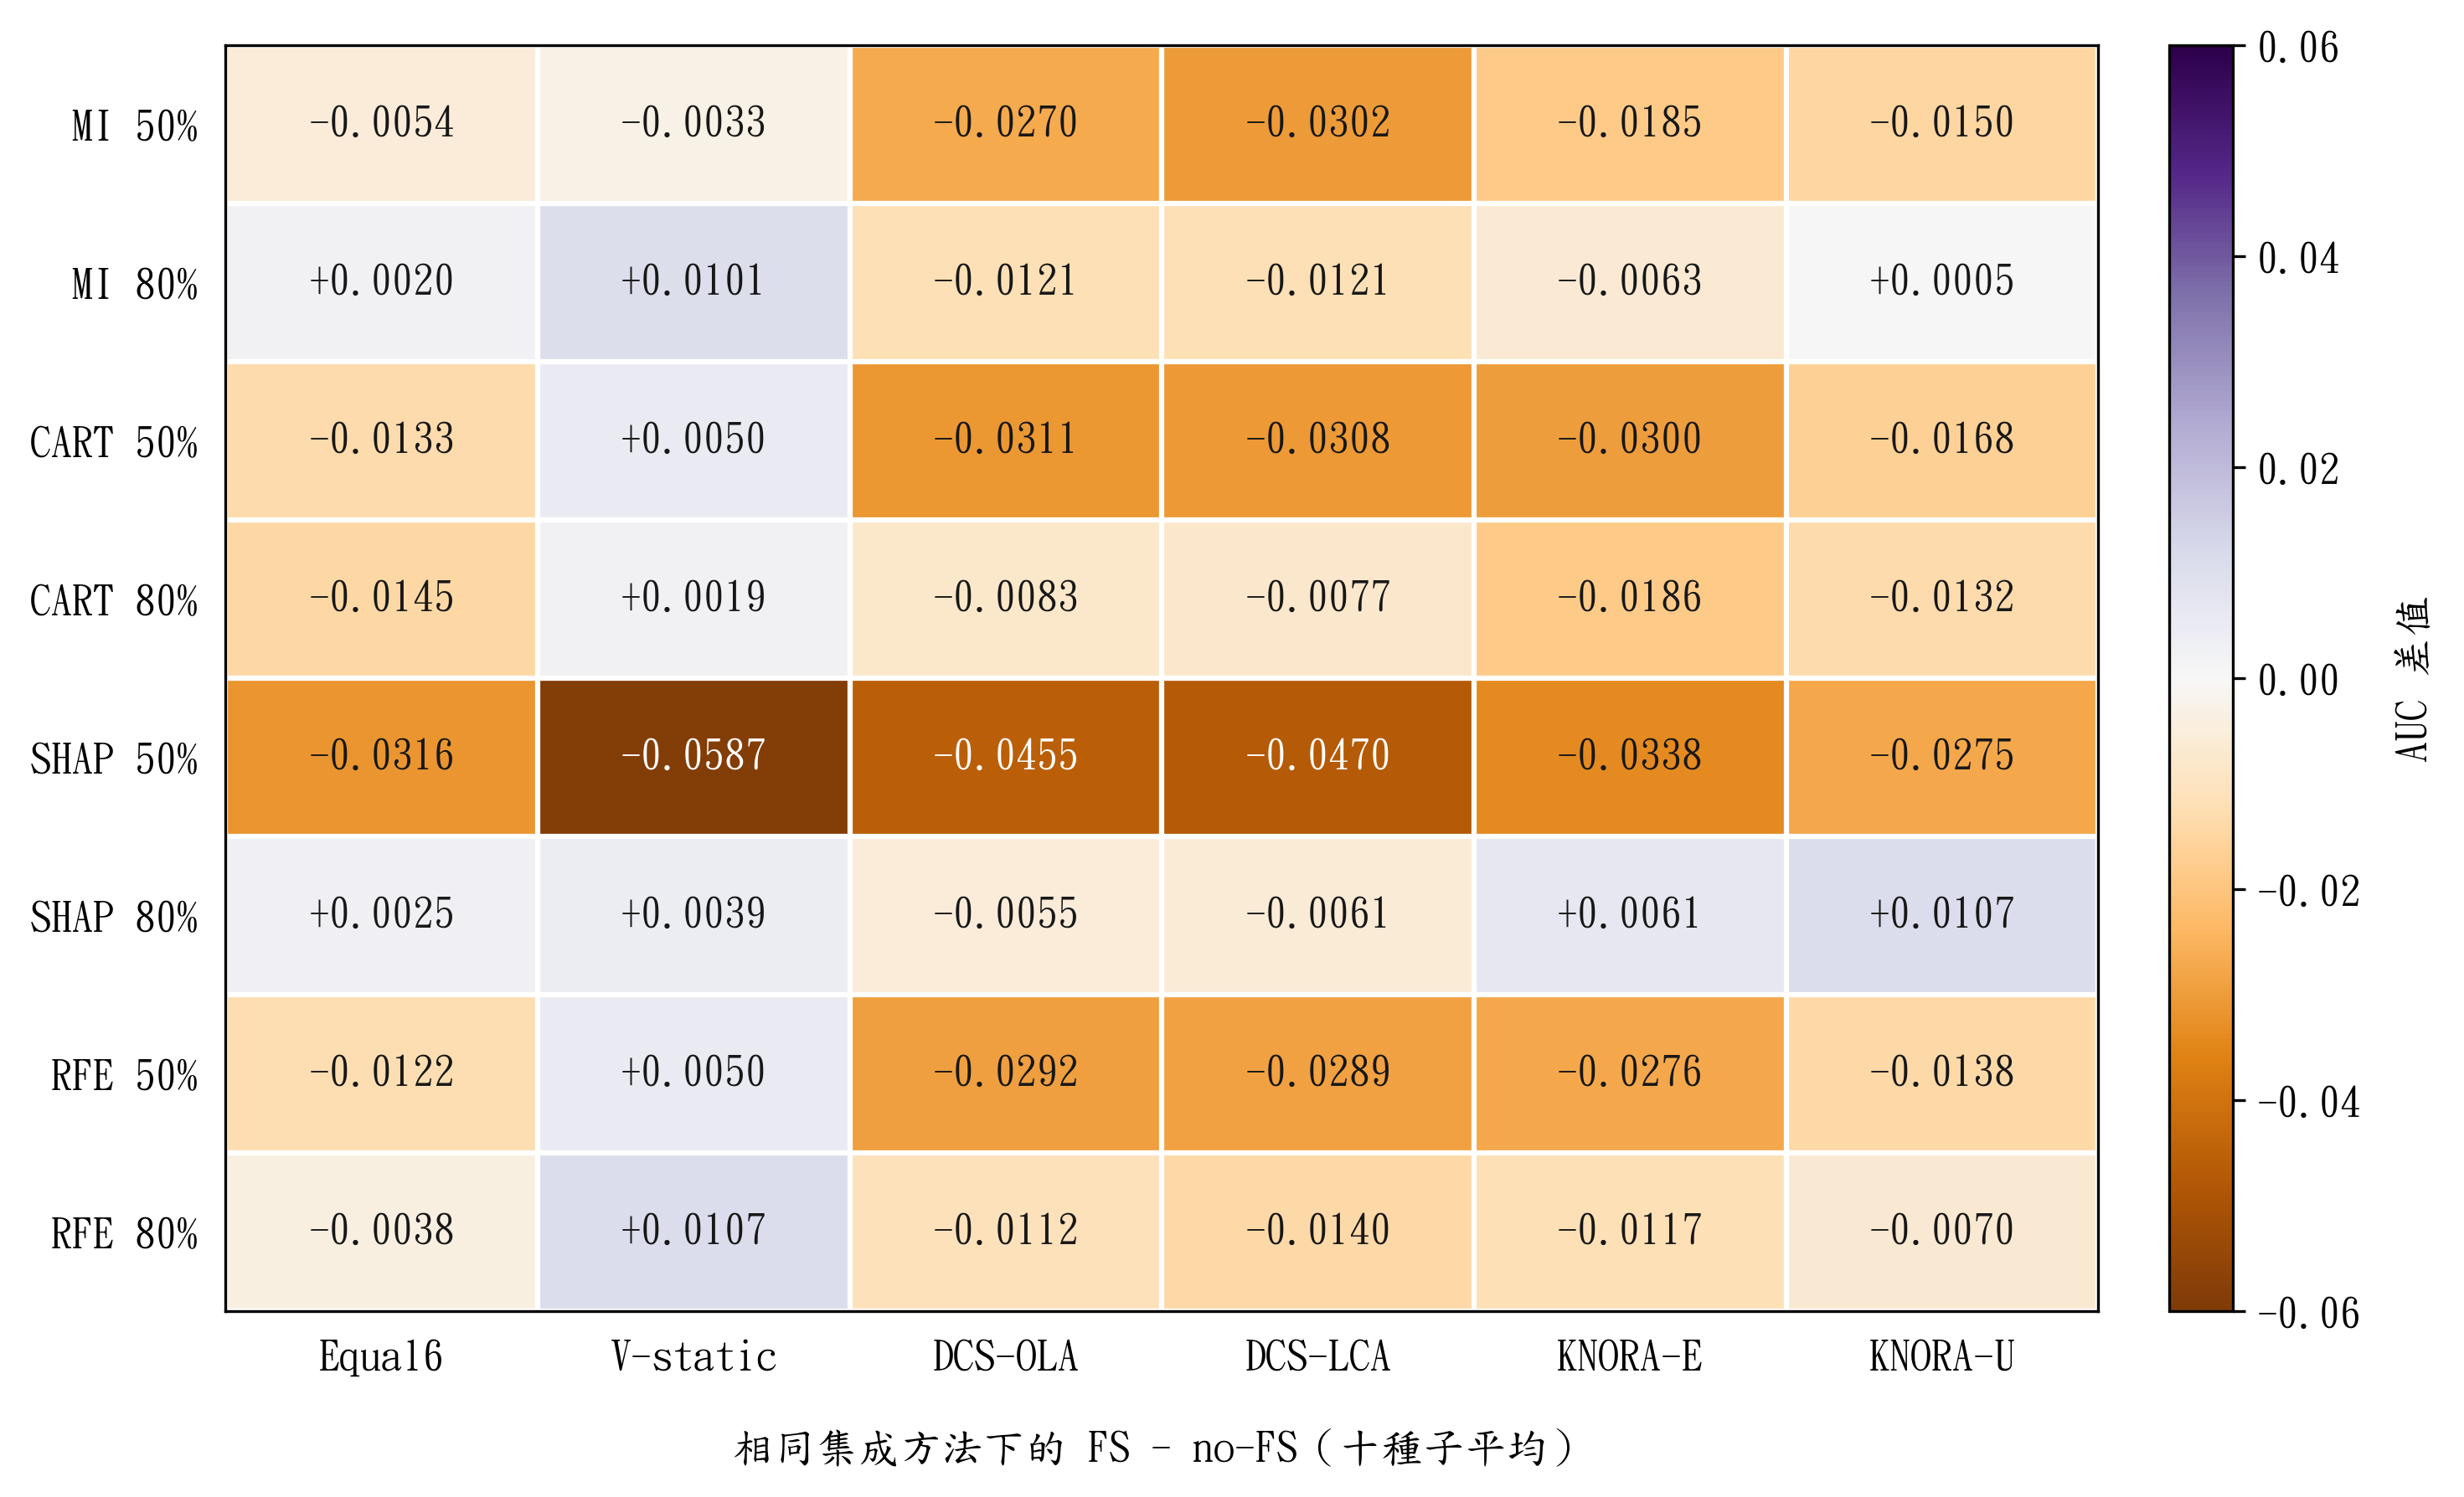
\includegraphics[width=\linewidth]{figures/event-fs-auc-differences.png}
\caption{事件標籤下各 FS 條件相對同方法 no-FS 之 AUC 差值}\label{fig:results-fs-differences}
\par\smallskip{\footnotesize (資料來源：本研究事件標籤 FS 集成實驗結果)\par 每格為十種子平均的 FS 減 no-FS，正值表示增加、負值表示下降。色彩只表示差值方向與大小，不表示統計顯著；50\%／80\% 分別實際保留 9／14 個特徵。\par}
\end{figure}

圖~\ref{fig:results-fs-differences} 顯示，多數 FS 條件降低 Equal6 與四種動態方法的 AUC，其中 SHAP 50\% 在六種方法都下降，降幅介於 0.0275 與 0.0587。V-static 在六個條件下 AUC 略增，最大為 RFE 80\% 的 0.0107；Equal6 與 KNORA-U 在 MI 80\% 與 SHAP 80\%、KNORA-E 在 SHAP 80\% 也有小幅增加。整體而言，保留 14 個特徵的條件較接近 no-FS，刪去一半特徵時下降較多。

F1-score 與 Recall 的方向依方法而異。V-static 在八個 FS 條件下的 F1-score 都低於 no-FS，降幅介於 0.0046 與 0.0399。Equal6 的 Recall 在八個條件都提高，增幅介於 0.0857 與 0.3244；兩種 DCS 則全部下降，但其 no-FS Recall 的種子標準差已超過 0.25，差值不宜單獨解讀。V-static 在 FS 後會重新選擇成員，例如 MI 50\% 只有五個種子仍選 Old\_under 與 New\_under，SHAP 50\% 只有四個種子，因此其變化包含整個選模流程，而非只反映特徵減少。

本實驗未出現在多數方法與指標上一致改善的 FS 條件。FS 能把輸入由 18 個減為 9 或 14 個，但需要接受 AUC 或 F1-score 的變動；是否可接受取決於應用對精簡程度與漏判、誤報的權衡。各特徵在十個種子中的入選次數列於附錄~\ref{sec:appendix-data-fs}。

\section{標籤定義對結果的影響}\label{sec:results-label}

為了解結論是否依賴標籤定義，表~\ref{tab:results-label-comparison} 對照相同資料列、模型池與選擇規則下，最終狀態標籤與事件標籤的 no-FS 結果。兩者正類比例不同，原始分數只比較方向，不比較高低。

\begingroup
\small\setstretch{1.12}\setlength{\tabcolsep}{3pt}
\setlength{\LTleft}{\fill}\setlength{\LTright}{\fill}
\Needspace{24\baselineskip}
\begin{longtable}{@{}>{\raggedright\arraybackslash}p{0.22\linewidth}>{\raggedright\arraybackslash}p{0.18\linewidth}>{\raggedright\arraybackslash}p{0.18\linewidth}>{\raggedright\arraybackslash}p{0.18\linewidth}>{\raggedright\arraybackslash}p{0.18\linewidth}@{}}
\caption{兩種標籤定義下未進行 FS 之集成結果}\label{tab:results-label-comparison}\\
\toprule
方法 & 標籤 & AUC & F1-score & Recall \\
\midrule\endfirsthead
\multicolumn{5}{c}{表~\thetable（續）}\\
\toprule
方法 & 標籤 & AUC & F1-score & Recall \\
\midrule\endhead
\midrule\multicolumn{5}{r}{續下頁}\\\endfoot
\bottomrule\endlastfoot
Old3 & 最終狀態 & 0.7134 & 0.1168 & 0.2383 \\
 & 事件 & 0.7198 & 0.0199 & 0.0168 \\
New3 & 最終狀態 & 0.7959 & 0.2007 & 0.2268 \\
 & 事件 & 0.8601 & 0.1289 & 0.4319 \\
Equal6 & 最終狀態 & 0.7815 & 0.1815 & 0.2690 \\
 & 事件 & 0.7881 & 0.1041 & 0.1941 \\
V-static & 最終狀態 & 0.8152 & 0.2355 & 0.2481 \\
 & 事件 & 0.8472 & 0.1795 & 0.2353 \\
DCS-OLA & 最終狀態 & 0.7386 & 0.1542 & 0.2909 \\
 & 事件 & 0.7450 & 0.0411 & 0.3857 \\
DCS-LCA & 最終狀態 & 0.7369 & 0.1631 & 0.3195 \\
 & 事件 & 0.7450 & 0.0404 & 0.3849 \\
KNORA-E & 最終狀態 & 0.7613 & 0.1837 & 0.2714 \\
 & 事件 & 0.7859 & 0.1017 & 0.2739 \\
KNORA-U & 最終狀態 & 0.7481 & 0.1817 & 0.2620 \\
 & 事件 & 0.7771 & 0.0686 & 0.4824 \\
\end{longtable}
\noindent{\footnotesize (資料來源：本研究固定年份集成實驗結果)\par 兩種標籤使用相同資料列、分區、模型池、十個種子與選擇規則；Test 正類分別為 287 筆（最終狀態）與 119 筆（事件）。正類比例不同，原始分數只比較方向，不比較高低。}
\endgroup


兩種標籤下，V-static 的 F1-score 都高於 Equal6，Old3 的 AUC 都最低，動態方法的 AUC 與 F1-score 也都未超過 V-static。差別在於最佳 AUC：最終狀態標籤下 V-static 為 0.8152，高於 New3 的 0.7959；事件標籤下則是 New3 的 0.8601 高於 V-static 的 0.8472。Old3 的 F1-score 也由 0.1168 降為 0.0199。最終狀態標籤把破產公司的每個年度都記為正類，歷史模型可以學到「哪些公司最終會破產」的特徵；改為只標記事件前一年後，歷史模型對近期事件的辨識能力明顯較弱。

最終狀態標籤已完成以公司為單位的配對 bootstrap 與 165 項 Holm 校正。該分析中，V-static 相對 Equal6 的 AUC 與 F1-score 增加均達校正後顯著（\(p_H\) 為 0.00632 與 0.02416），FS 則沒有校正後顯著的 AUC 增加；完整結果見附錄~\ref{sec:stats-full}。這些檢定只適用於最終狀態標籤，不直接延伸至事件標籤。

\section{研究問題的綜合討論}\label{sec:results-discussion}

\subsection{訓練資料期間與單一分類器}

研究問題一的答案是：資料期間的效果依分類器而異。XGBoost 與 LightGBM 以 New 的 AUC 較高，Random Forest 以 Retrain 最高，Logistic Regression 三者相近。由於各策略的訓練筆數同時不同，本研究不把差異完全歸因於資料新近程度。

\subsection{集成規則與模型成員}

研究問題二的答案是：在固定的預設參數模型池中，成員選擇比整合方式更重要。New3 與 V-static 優於 Equal6 及四種動態方法；兩者分別以 AUC 和 F1-score 較高。歷史模型在事件標籤下表現較弱，V-static 只保留最好的 Old 模型，Equal6 全部納入則降低排序能力。此結果支持保留簡單的單一期間與等權控制組，再以驗證資料決定是否加入歷史模型。

不過，調參後的單一分類器與集成表現相當，集成池成員又未經調參。因此本研究只能說明同一池內整合方式的差異，尚不能主張集成優於調參後的單一模型。

\subsection{特徵精簡與少數類辨識}

研究問題三的答案是：FS 沒有帶來一致的改善。保留 14 個特徵時大多接近 no-FS，保留 9 個特徵時 AUC 多半下降；Recall 與 F1-score 的方向則隨集成方法而變。本研究記錄了特徵數，但未比較訓練與推論時間，因此不能將輸入維度減少換算為已證實的成本節省。

\section{推論範圍與限制}

事件標籤以破產公司的最後觀測年度推定事件時間，並非逐筆核對的破產申請日；Calibration 與 DSEL 各只有 16 與 17 筆事件，選模與門檻決策的不確定性較大。事件標籤結果尚未完成配對檢定，本章差異均為描述性。同一公司可能同時出現在擬合與測試期間，主要實驗也採固定年份、測試期間不更新模型，因此結果不代表對未見公司或持續學習情境的驗證。實證只使用一份公開資料，結論限於本資料與既定時間分區。
\endgroup
